% pap/ssb-icn2019-paper/main.tex

\documentclass[9pt,sigconf]{acmart}

% \usepackage{showframe}

% XXX there are brittle hacks to render the first page layeout inside
% the given margins (when showing the CC-BY-SA logo and text)

\title[Secure Scuttlebutt: An Identity-Centric Protocol
       for Subjective and Decentralized Applications]{%
  Secure Scuttlebutt: An Identity-Centric Protocol \\
  for Subjective and Decentralized Applications
}

\author{Dominic Tarr}
\affiliation{ssb:@EMovhfIrFk4NihAKnRNhrf}
\email{RaqIhBv1Wj8pTxJNgvCCY=.ed25519}

\author{Erick Lavoie}
\affiliation{McGill University, Montreal, Canada}
\email{erick.lavoie@mail.mcgill.ca}

\author{Aljoscha Meyer}
\affiliation{TU Berlin, Germany}
\email{aljoscha.t.meyer@campus.tu-berlin.de}

\author{Christian Tschudin}
\affiliation{University of Basel, Switzerland}
\email{christian.tschudin@unibas.ch}

\acmYear{2019}
\acmConference[ICN '19]{6th ACM Conference on Information-CentricNetworking}{September 24--26, 2019}{Macau, Macao}
\acmBooktitle{6th ACM Conference on Information-Centric Networking (ICN '19),September 24--26, 2019, Macau, Macao}
\acmDOI{10.1145/3357150.3357396}
\acmISBN{978-1-4503-6970-1/19/09}

\copyrightyear{2019}
\setcopyright{rightsretained}
\renewcommand{\copyrightpermissionfootnoterule}{%
  \vspace*{-2ex} % XXX hack
  \kern-3pt\hrule width \columnwidth \kern 2.6pt%
  \noindent%
  
\includegraphics[width=0.25\columnwidth]{figs/creative-commons-by_sa_4_0.pdf}
  \hspace*{-2pt}
  \begin{minipage}[b]{0.74\columnwidth}
    \footnotesize
    For any reuse or distribution, you must make clear to
    others the license terms
    of this work. The best way to do this is with a link to the web page
    http://creativecommons.org/licenses/by-sa/4.0/%
    \hspace*{-1pt}
    \vspace*{-1pt}
  \end{minipage}%
  \vspace*{2pt}%
  \kern-3pt\hrule width \columnwidth \kern 2.6pt%
  \vspace*{-2pt}
}

\begin{CCSXML}
<ccs2012>
<concept>
<concept_id>10003033.10003034</concept_id>
<concept_desc>Networks~Network architectures</concept_desc>
<concept_significance>500</concept_significance>
</concept>
<concept>
<concept_id>10011007.10010940.10010971.10010972.10010975</concept_id>
<concept_desc>Software and its engineering~Publish-subscribe / event-based architectures</concept_desc>
<concept_significance>500</concept_significance>
</concept>
<concept>
<concept_id>10010520.10010521.10010537.10010540</concept_id>
<concept_desc>Computer systems organization~Peer-to-peer architectures</concept_desc>
<concept_significance>300</concept_significance>
</concept>
<concept>
<concept_id>10002951.10003152.10003161.10003162.10003414</concept_id>
<concept_desc>Information systems~Linked lists</concept_desc>
<concept_significance>300</concept_significance>
</concept>
</ccs2012>
\end{CCSXML}

\ccsdesc[300]{Networks~Network architectures}
\ccsdesc[300]{Software and its engineering~Publish-subscribe / event-based architectures}
\ccsdesc[300]{Computer systems organization~Peer-to-peer architectures}
\ccsdesc[300]{Information systems~Linked lists}

\keywords{Secure Scuttlebutt, Information-Centric Networking, Push vs.~Pull}

% ----------------------------------------------------------------------
\begin{document}

\begin{abstract}
  Secure Scuttlebutt (SSB) is a novel peer-to-peer event-sharing
  protocol and architecture for social apps. In this paper we describe
  SSB's features, its operations as well as the rationale behind the
  design. We also provide a comparison with Named Data Networking
  (NDN), an existing information-centric networking architecture, to
  motivate a larger exploration of the design space for
  information-centric networking primitives by formulating an
  identity-centric approach. We finally discuss SSB's limitations and
  evolution opportunities.
\end{abstract}

\maketitle


% ----------------------------------------------------------------------

\section{Introduction}

A simple conceptual architecture for community applications consists
of a global data pool to which every person can contribute and where
every person can tap into the shared data~-- data sharing being the
purpose of such applications. This model still is valid if one adds
access control to the picture, either tied to the data (encryption
giving access to content only to entitled holders of the decryption
keys) or encrypting data in transit (login and TLS). Facebook and
%
% XXX hack to make the additional CC license box fit into the ACM footer
\makebox[\columnwidth][s]{%
  other centrally organized social app service providers fit well under
}\\
\ 

\noindent
this global data pool model but have been strongly criticized for
abusing their central provisioning position.  The ``decentralized
web movement''~\cite{decent-2018-aug} is the most visible technical
response to this critique, pointing out implementation alternatives.

One of these alternatives is a project called Secure Scuttlebutt (SSB)
that started in 2014. After several iterations of protocol design and
implementation, SSB has become a stable service for over 10,000 users
offering them rich media community applications with strong
cryptographic protection (end-to-end encryption and metadata privacy)
and running in pure peer-to-peer mode.

\subsection*{Selective Complete Log Replication}

SSB relies on the core insight that each participant is only
interested in a \textit{subset} of the global data pool, thus it is
feasible to locally store all the data a participant is interested
in. To partition the data pool, all data is associated with the
\textit{identity} that produced it. Participants select their slice of
the data pool by specifying the set of identities whose data they care
about. This creates a ``social graph'' along whose edges data flows
(Figure~\ref{fig:net-of-people}). Even as the overall system scales,
the amount of data any single peer is interested in and thus needs to
handle stays roughly the same.

Each participant can publish data to their single-writer, append-only
log. This choice of data structure allows efficient replication and
verification of the integrity of received data. Replicating these
larger slices of the data pool comes with an unusual set of tradeoffs,
discussed throughout the paper. As it turns out, replicated logs form
a solid foundation for implementing many classes of applications.

\begin{figure}[htb]
  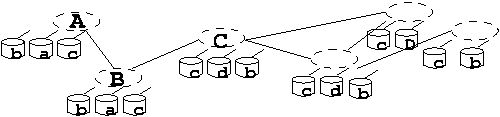
\includegraphics[width=0.9\columnwidth]{figs/net-of-people.pdf}
  \caption{SSB's ``Internet of Identities'' -- {\rm\small Users A, B
      and C replicate logs ({\em a, b, \ldots}) based on whom they
      follow: {\em C} does not follow {\em A}, hence has no log {\em
        a}. {\em A} and {\em B} follow each other such that when {\em
        A} follows {\em C}, {\em A} will get {\em C's} log {\em c} via
      {\em B:} new content is pushed directly if possible and through
      intermediary friends if necessary.}}
  \Description{Explaining SSB as an ``Internet of Identities'' where
    humans connect to each other and replicate their friends' content.}
  \label{fig:net-of-people}
  % XXX hack to reduce space to next section title
  \vspace*{-2ex}
\end{figure}


\subsection*{Subjective Reader}

Because replication in SSB is selective and driven by a peer's
social graph, different end devices will have access to different sets
of log replicas, leading to different views of the world, which we call
a ``subjective reader'' approach. SSB considers this a desirable
property: each peer is free to
consider data sources of its own choosing instead of having to feed
from a centrally provisioned or otherwise converged view. While it is
possible to implement consensus protocols over SSB, or to designate
central data aggregators from which many peers consume the
consolidated outputs, the SSB network itself deliberately doesn't
offer consensus services nor central content (directories etc). In
Section~\ref{ssect:dapps} we will show the implications of this
technological choice on the structure of distributed applications that
can only read from and write to local logs.

\subsection*{Novelty}

Putting complete replication of individual append-only logs at the
core of SSB's protocol avoids several hard problems in distributed
systems. {\bf First}, it is a radically decentralized approach
requiring only minimal specification-level coordination among the
participants but no run-time checks or configuration management.
%
{\bf Second}, although append-only data structures are well known for
their benefits and are at the core of crypto currencies' consensus
finding, SSB uses logs without any consensus properties. The issue is
deliberately sidestepped, but all necessary building blocks are
provided to higher layers.
%
{\bf Third}, crafting a cryptographic ID system and maintaining a
social graph that informs routing creates a very narrow filter: it
implements a receiver-driven approach where data only flows where it
is needed and provides flexibility in the actual data dissemination
strategy.
%
{\bf Fourth}, it makes every peer a publisher by design. This property
goes beyond the decentralized approaches like DAT~\cite{datproject} or
IPFS~\cite{benet2014ipfs} which assume that there exist replication
servers but keep the separation between a data transport network and a
server layer.
%
{\bf Last but not least}, log replication leads to a distributed
system with inherent high resilience as any communicating element
carries a persistent copy of the data. In traditional distributed
systems, coordinating the data persistence as a basis for resilience
is often an add-on task, or requires at least a special recovery
service.

\subsection*{Comparing SSB to NDN}

Despite SSB data replication being currently implemented as an
application protocol (layer 7 in the OSI
stack~\cite{briscoe2000understanding}), we believe that its underlying
principles are worth studying from a network API perspective (layer 3
in the OSI stack) to highlight regions of the design space that could
be further investigated. We sketch here some aspects in which SSB
differs from \textit{Named Data Networking}
(NDN)~\cite{ahlgren2012survey}, a popular proposal for
Information-Centric Networking (ICN). A longer exposition of SSB's
underlying communication model is available in a separate
publication~\cite{tschudin2019broadcast}.

In SSB, the delivery of information is organized around \textit{named
  data streams} for signed events. The basic unit of addressing is a
full log that might still produce new event messages in the future.
The SSB streams guarantee \textit{reliable causal
  ordering}~\cite{cachin2011introduction} and \textit{authenticity}.

Delivery of streams follows a \textit{push model}: once a receiver has
expressed interest in a stream, new items are transferred
automatically without being requested individually. Flow-control
(back-pressure) in the current overlay implementation is done
implicitly by the TCP connections used to deliver data among peers.

Streams are tied to a single \textit{identity} with a corresponding
\textit{public key}\/: only this identity can produce new items in the
stream with the correct signature.  Because the signature ensures the
integrity of the items, they can be served from anywhere and by
anybody.
%
Moreover, users independently create the key that serves as an
identity. Streams are therefore
\textit{self-certifying}~\cite{mazieres1998selfcertifyingpathnames}
and their integrity does not rely on an external trust anchor nor a
central naming authority or other name coordination and allocation
mechanisms.

In contrast, NDN embodies quite different design choices. First, the
basic elements of networking are \textit{single pieces of data},
identified by hierarchical names similar to paths in a
filesystem. Second, data is accessed via a \textit{pull} model: a
consumer issues an \textit{interest} in a name, and the network
delivers the corresponding data. Third, many NDN schemes rely on a
hierarchical trust model to issue certificates that can in turn be
used to sign individual pieces of
data.\footnote{See~\cite{zhu2012chronos} for a proposal that leverages
  a web of trust model in a decentralized chat application built on
  top of NDN.}

It is not clear that either design can subsume the other: one can
implement SSB over NDN or the opposite but each option comes with
significant runtime costs. Still, there could be an intermediate
territory where a future synthesis of the two approaches may
emerge. We therefore analyze the trade-offs that appear in various
ways of layering NDN and SSB to enrich the discussion around future
developments in ICN.

\subsection*{Structure of this paper}

We start out by giving an overview of the SSB protocol in Section
\ref{sect:architecture}. Next we describe common patterns of how
applications can be built on SSB (Section \ref{sect:apps}). We show
how SSB relates to other networking protocols, first through a
detailed comparison with NDN (Section \ref{sect:NDN}) and then in the
broader context of related work (Section \ref{sect:relwork}). We
conclude the paper with an outlook on some of the ``work in progress''
(Section \ref{sec:wip}) and an evaluation of the problems (Section
\ref{sect:nay}) and benefits (Section \ref{sect:yay}) of the SSB
approach.


% ----------------------------------------------------------------------

\section{SSB Architecture and Protocol}
\label{sect:architecture}

In SSB, each user is identified by an ed25519~\cite{bernstein2012high}
keypair. Since anybody can generate a random keypair with very low
probability of multiple peers generating the same keypair, no central
authority is necessary for introducing users to the
system. Conceptually, SSB is a network of identities that connect to
each other (physical topology) and share mutual or unilateral interest
in the other peer's data (social graph), as shown in
Figure~\ref{fig:net-of-people}. A node running the SSB protocol is
called a \textit{relay}. The identity that holds the private key of a
log is called its \textit{author}.

The {\em single-writer append-only logs} of SSB consist of entries
(called \textit{messages}) that include a {\em backlink} in the form
of a cryptographic hash of the previous message (or a special
indicator for the first message of a log). The most distinguishing
feature of this linked list, when compared to a regular blockchain, is
that each SSB user maintains their own log and cryptographically signs
all their (and only their) messages. Messages whose backlink points to
a message in a different log (i.e. by a different author) are
considered invalid and will be rejected by SSB relays.

These constraints still allow creation of arbitrary trees rather than
logs. To enforce log structure, each SSB relay checks that every
message has exactly zero or one incoming backlinks. If it has more
than one, the log is considered {\em forked}. All messages from the
point of the fork onwards are ignored, the log cannot be appended to
anymore.

Concretely, each message, which may not exceed 4 KB, contains the
following pieces of data~\cite{ssb-spec-messages}:

\begin{itemize}

\item the {\em backlink} to the previous message, or a null value

\item the public key of the message's {\em author}

\item the {\em sequence number} of the message, which must be one more
  than the sequence number of the previous message, or exactly one if
  it is the first message of the log

\item a claimed {\em timestamp} of when the message was created

\item a {\em hash} indicator that specifies the concrete hash function
  that was used to compute the backlink

\item the {\em content} of the message

\item the author's {\em signature} over all the previous data

\end{itemize}

In the current version of SSB, {\em content} is a JSON object that
must contain a {\em type} key that serves as a hint for how the
content should be interpreted. SSB enforces that the content is valid
JSON by rejecting any malformed message.  Encrypted content is
represented as a base64-encoded string, together with a tag that
signifies which encryption algorithm was used.

SSB defines a format for encoding specifically the public keys of
identities and the hashes of messages and blobs (see below) as
strings. This allows applications to scan the content of messages from
other authors for such references, e.g. in order to create database
indices (see Sect.~\ref{ssect:dapps}).

\subsection*{Replication}

The principal function of SSB relays is to connect to other relays and
exchange log {\em updates}. To do so, relays maintain a point-to-point
encrypted~\cite{tarr2015secrethandshake} overlay network over which
they run a gossip protocol. When two relays start gossiping, they
exchange the current sequence numbers of all logs they are interested
in. If a relay receives a lower sequence number for a log than it
sent, it transmits the messages that the other relay is lacking. If at
a later point a new message of the log becomes available to a relay,
it is automatically \textit{pushed} to the connected relays. As an
optimization, this {\em eager} gossip is only performed over the edges
of a spanning tree, which itself is maintained via the
plumtree~\cite{leitao2007epidemic} protocol. In classic peer-to-peer
fashion, clients (leaf nodes) are no different than relays except that
they usually include some graphical user interface and perform
application logic.

In addition to this primary replication mechanism, SSB provides two
other ways of exchanging information. {\em Blobs} are
content-addressed pieces of free-form data, typically images or other
documents larger than the 4KB limit, that are referenced from messages
but are not part of any log. They are not widely disseminated
automatically, but rather fetched on demand via a simple
request-flooding protocol. {\em Out-of-order messages} are a similar
mechanism to address and fetch messages on demand via their hashes.

\subsection*{SSB Relays as an Application Platform}

Beyond replicating logs and checking the validity of update messages,
an SSB relay offers an API to its peers. Peers can host arbitrary
programs that issue remote procedure calls (RPCs) to the relay. The
exposed functionality includes appending to a log (if you know its
private key), reading from logs, requesting which logs a relay should
replicate, and fetching blobs and out-of-order messages.

The reference implementation of the SSB relay~\cite{ssb-server},
written in JavaScript, also includes a mechanism for loading {\em
  plugins} into the relay to extend its functionality. There are a few
default plugins: conceptually these can be thought of as client
programs that are always running. Of particular importance are those
that guide the replication process. The {\em friends}
plugin~\cite{ssb-friends} scans the relay's log for specific messages
that indicate which other identities the author {\em follows}. The
plugin then instructs the relay to fetch and replicate these
logs. These other logs might of course also contain some of these
messages. The friends plugin transitively replicates these
friends-of-a-friend logs as well, up to a configurable maximum
distance in the friends graph.

Beyond ``befriending'' other authors through {\tt follow} messages
(i.e. messages of type {\tt follow}), an SSB user can control the
shape of their social graph via special {\tt block} messages which
limit the transitive log replication. Both the {\tt follow} as well as
{\tt block} messages are overheard by relays, through scanning all
received log updates, and inform them about where updates should be
delivered (or not). Decisions about whom to replicate can be --and in
the current system is-- guided by the content of the very data that is
replicated. By storing the relevant information inside the author's
log (as opposed to a local or central database), other peers can use
this informtion to guide their decisions.

The overlay network also makes use of logs to store configuration
information, in this case the SSB\_ID-to-IP\_address mapping:
operators publish the static IP addresses of highly-available relays
(called {\em pubs}) to their log. When an SSB relay needs to connect
to the overlay, the responsible plugin can scan any locally available
log replica for this information.

\subsection*{SSB's Layered Architecture}

It is worth noticing that SSB spans three independent layers of
protocols. The most fundamental protocol is the message format: all
peers need to agree on what constitutes identities, valid messages,
and how to compute hashes to address messages and blobs. This is the
``thin waist'' of SSB (see figure~\ref{fig:waist}).

\begin{figure}[htb]
  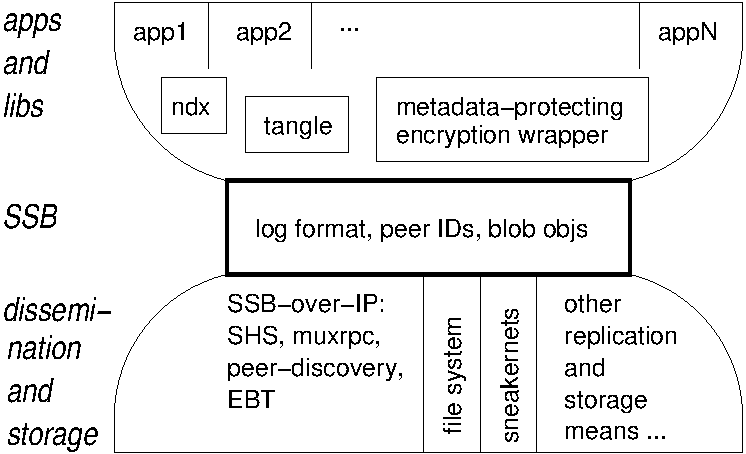
\includegraphics[width=0.9\columnwidth]{figs/ssb-waist.pdf}
  \caption{Secure Scuttlebutt's protocol stack.}
  \Description{Secure Scuttlebutt's protocol stack.}
  \label{fig:waist}
\end{figure}

Next (below) is the specific mechanism by which relays exchange
data. The default RPC mechanism is one option, but alternative
mechanisms such as distribution via a sneakernet could also be
used. Different peers that do not share a common replication mechanism
could still interact indirectly, as long as there are some relays that
understand multiple replication protocols.

In other words, the core logical replication protocol by which a relay
serves its clients is fully independent from the actual dissemination
protocols. And finally, the publishing and interpretation of
application data in such messages is again a separate affair that is
layered on top of the thin waist.


% ----------------------------------------------------------------------

\section{Distributed Apps and Data Structures over SSB}
\label{sect:apps}

The replication model of SSB enables many collaborative applications
to be implemented easily by abstracting much of the complexity in
distributing the updates. However, implementing such applications
still comes with challenges. To introduce them, we first discuss in
detail the implementation of a user directory to introduce the
implementation approach, then briefly cover other applications
currently in use, and finally discuss some core issues that are shared
between all applications.

\subsection{Example: SSB's user directory}
\label{ssect:about}

`{\small\tt about}' is SSB's user database i.e., an application that
associates cryptographic IDs with (typically) human-readable
attributes. A single message format has been defined to this end:
%
{\small\begin{verbatim}
'content': {
  'type'  : 'about',
  'about' : about_id,
  attr_name : attr_value   // multiple times
}
\end{verbatim}}

\noindent
The {\small\tt about} app scans all logs for messages of type
{\small\tt `about'} and constructs a database as shown in
Figure~\ref{fig:about}, retaining the most recent attribute assignment
found. In this database, an {\small\tt about\_id} is associated with a
list of key/value pairs which are prepended by the publishing author's
ID. It is left to the end user's {\small\tt `about'} application to
subjectively select which of these bindings should be displayed.
%
Currently the {\small\tt name}, textual {\small\tt description} and
{\small\tt image} attributes are understood by most SSB user
interfaces and are used to substitute or decorate the cryptographic
ID. If {\small\tt about\_id} and {\small\tt author\_id} are identical,
this means that an attribute was self-chosen and then is usually
rendered with a higher preference over key/value pairs assigned by
others.

\begin{figure}[htb]
  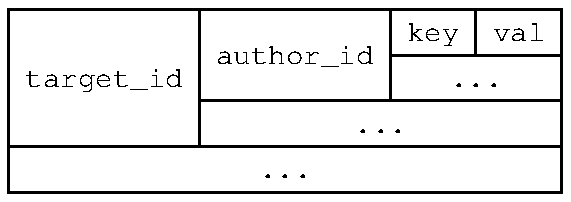
\includegraphics[width=0.6\columnwidth]{figs/about-ds.pdf}
  \caption{SSB's user directory data structure (after extraction from
    the logs).}
  \Description{SSB's user directory data structure shown as a record.}
  \label{fig:about}
\end{figure}

\noindent
In terms of CRUD\footnote{Create, Read, Update, Delete} actions,
creation happens once a new SSB identity adds its own {\small\tt
  about} message to its log; reading the user database is performed on
the above data structure; updates are expressed by adding an
{\small\tt about} message --regardless whether it relates to the
author itself or to another identity-- to one's own (!) log and all
peers updating their extracted database; deleting a user entry is not
possible, at least not directly (one would have to block that user ID
as well as all IDs which wrote an update for that user).

There can never be confusion about the sequence or scope of attribute
assignments because they are orderd by the log (and thus in time) and
kept separate, per author ID. Note also the presence of the
``subjective reader'' property: the content of a peer's user database
is dependent on their position in the social graph. The ``subjective''
mindset is also visible by letting every user assign attributes to
anybody, leaving it to the user interface (and human viewer) to select
which of the self-chosen or given display names and images is most
suitable for a given ID.

\subsection{Profiles of other selected SSB apps}
\label{Section:AppProfiles}

Multiple applications have been written by contributors and are used
daily by the SSB community. The following selected examples represent
alternatives to well-known services and they illustrate both
opportunities and challenges of communication through replicated
append-only logs.

\textit{Git-ssb}~\cite{git-ssb} is an alternative to
GitHub~\cite{github} that replicates git-based version-controlled code
repositories through contributors logs. It provides an encoding of
repositories in SSB logs, a bridge to interoperate with git
repositories, and a web-based viewer to browse repositories. The
object model of Git~\cite{chacon2014pro} has a similar structure to
SSB's logs. Other git operations, such as creating repository, are all
SSB messages. Since any user can independently update the
\textit{same} repository, as defined by its creation message,
consensus on the ``official'' master branch and its latest commit is
enforced through social coordination. In case of concurrent updates to
the same branch in the same repository~\cite{git-ssb-push-conflict},
referencing both concurrent updates in a later merge commit in effect
resolves the ambiguity.

\textit{Ssb-chess}~\cite{ssb-chess} is a correspondence chess
application in which players can invite one another to play,
alternatively share their next move until the game ends, and external
observers can comment on the game.  Because the rules of chess
preclude concurrency, i.e. at any time there is always only one of the
two participants that is permitted to modify the state of the chess
board, a game can easily be represented as a linked list with nodes
representing chess moves alternating between the two participants'
logs.  Moreover only the participants, explicitly mentioned in the
original invitation, are allowed to modify the state of the game. The
implementation does not require concurrency management and is
therefore conceptually straight-forward.

\textit{Gatherings}~\cite{patch-gatherings} are alternatives to
Meetup~\cite{meetup.com} that enables participants to signal their
intention to attend or not attend to physical events. A gathering is
defined by its creation message but otherwise has no fixed
properties. Anyone that has a reference to the creation message may
change its properties, such as location, start and end dates,
description, and image, by publishing an update message. The value of
those properties are the most recent set by anyone. Initially, recency
was determined by the time of creation, as reported by the user's
client implementation (\textit{self-stated creation time}). To be more
robust to potential invalid timestamps however, some client
implementations have started using the time at which message updates
are \textit{received}, then disambiguate using the self-stated
creation time.

\subsection{Running Distributed Applications over Replicated Logs}
\label{ssect:dapps}

``Infrastructure-less'' distributed application as presented above
become possible because central servers can be fully replaced by each
peer working on its local set of replicated logs. In this subsection
we discuss the particularity of this approach and its constraints.

A common pattern of SSB's applications is that they heavily rely on
local database support for organizing the data contained in the logs.
Typically a map-reduce strategy is used where the map phase filters
the logs and the reduce actions computes the latest application state.

In the user directory application (Sect.~\ref{ssect:about}), the
filtering is done by selecting only {\tt about} messages for a
specific target ID and the reduce action consists in accumulating the
latest key-value pairs such that a more recent key-value pair replaces
an older one if it was signed by the same author\_id. The size of the
replicated logs, although locally stored, would lead to very long
response times if the map-reduce would be executed at
render-time. Instead, almost each application will build indexes and
aggressively cache state that was already aggregated. Should the
indexes ever become corrupted (e.g. because the user interface app
crashed in the middle of a complex indexing step), they can be fully
regenerated from scratch.

An important aspect is whether the reduction step can be done in an
incremental fashion by reusing previously computed application state.
For example, counting the ``likes'' that a post receives works fine:
incoming log extensions are indexed and if they are of the like type,
the counter corresponding to the referenced message is incremented.

Other applications, however, may need a {\em full} re-evalution of the
reduce function each time the underlying index changes. An example for
this case is a chat in form of sequence of post messages: if some
identity is added to the set of followed identities, its log is
incrementally replicated, and so are the posts of this identity. For
each incoming new post, which may have been written very long ago, one
has to insert it at the right place. This problem is shown in
Figure~\ref{fig:tangle} where a message has not yet been replicated to
a client and, once it arrives, has to be properly inserted into the
application-level data structure.

\begin{figure}[htb]
  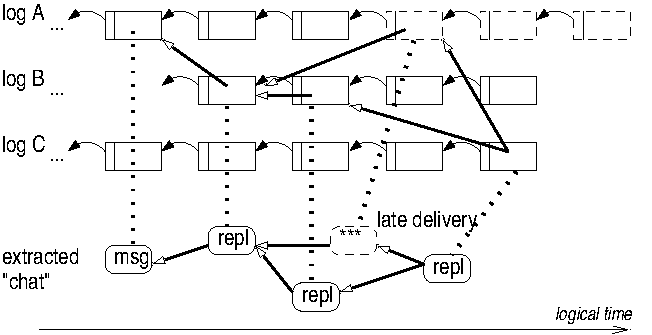
\includegraphics[width=0.9\columnwidth]{figs/tangle.pdf}
  \caption{Example of extracting application data spread over multiple
    collaborating logs and dealing with not-yet-delivered data.}
  \Description{Extracting a discussion thread from multiple collaborating logs.}
  \label{fig:tangle}
\end{figure}

A simple solution (adopted in some SSB client software) is to use the
timestamp claimed by the author of the post, and in this case one can
reuse the existing time-sorted list and insert the new post. However,
because an author could lie about the timestamp, the reduce function
should do a topological sort based on the causality relationship with
other posts and their replies, which form a directed acyclic graph.%
%
\footnote{Writers can facilitate the causal ordering by explicitly
  referring to the most recent messages in other logs they were aware
  of at the time of writing, regardless of whether the content was
  directly relevant to their own message. We call the graphs resulting
  from this pattern ``tangles''.}
%
Insertion into the dependency graph
may or may not lead to having to rerun the sort on the whole graph of
postings. Clearly, the lack of a central server hosting the reference
list of posts and being able to record a post's submission time, leads
to more complex client software that must prepare for and defend
against a broad range of adversarial data found in the logs.


\subsection{Synchronization and Eventual Consistency}
\label{Section:Tangle}

SSB's basic log replication service synchronizes peers in a consistent
way: due to the hash chaining, events (represented by messages in a
log) will be delivered in the order they happened and replica content
will be consistent. This does not instantly lead to consistent shared
data structures, though, if the corresponding events are spread over
multiple logs. Instead, the natural guarantee is that of {\em partial
  eventual consistency} where all peers will see the same reduced
application state {\em if they share the same log set} after
sufficient replication progress. Because of the eager, push-based
forwarding of messages, consistency can be reached quickly, even if
there is no end-to-end connectivity.

Eventual consistency is the hallmark of Conflict-free Replicated Data
Types (CRDTs, see~\cite{shapiro2011conflict}) which are directly
applicable to the SSB setting as they only assume a reliable and
(sometimes) in-order delivery of update messages. Potentially, CRDTs
permit to implement global data structures featuring eventual
consistency without coordination effort (thus are fully scalable). The
caveat here is that SSB peers do not necessarily see all involved logs
due to their position in the social graph which controls replication
wherefore consistency is always modulo that fact. For example, like
counts will be eventually consistent with respect to the same set of
followed authors but not globally, at least if they are directly
counted. Other applications relying on reduction via set union may
learn from state that stems from beyond the circle of followed
authors.

More research is needed to understand the constraints brought by the
combination of coordination-less interaction with partial log
replication, but SSB's rich set of applications used on a daily basis
is an encouraging sign that eventual consistency in combination with
subjective replication is a ``good enough'' basis for real
decentralized services.


% ----------------------------------------------------------------------

\section{Comparing SSB with Named Data Networking (NDN)}
\label{sect:NDN}

In this section, after a brief introduction to NDN we compare and
relate SSB to NDN in three different ways: layering SSB on top of NDN,
layering NDN on top of SSB, and a hybrid mode that combines features
of both. The purpose is to shed light on the sometimes implicit
assumptions behind SSB and NDN and show a larger design space for
future ICN developments.

\subsection{Named Data Networking}

NDN is an evolution of the Content-Centric Networking proposal that
was publicly presented by Van Jacobson in
2006~\cite{vanJacobson2006ccn}. Both aim to address shortcomings of
using the Internet Protocol (IP)~\cite{cerf1974protocol} for data
dissemination from a single source to a number of users. In the IP,
the routing layer only deals with the delivery of data packets from a
source to a destination, regardless of their content: when multiple
users request the same content from different machines, the routing
layer therefore has to deal with redundant data transfers and is prone
to content tampering by intermediate routing nodes. Some of the major
goals of NDN are therefore to optimize data distribution for large
content providers while guaranteeing the integrity of content. NDN
currently achieves those aims by: (1) initiating data transfers
\textit{after} the interested users are known by the network
(\textit{pull-model}), (2) leveraging \textit{existing certificate
  infrastructure} to authenticate the content, and (3) \textit{naming}
individual pieces of data, using a naming scheme that reflects the
hierarchical organization of major content providers, such as
universities, governments, and major media companies.

Technically, a receiver has to request content by name --in a so
called {\tt Interest} packet-- and at most one matching content is
returned in a corresponding {\tt Data} packet. The Data packet
includes the content's name and is signed such that a forwarding node
can verify the correctness of the name-to-content binding.

\begin{verbatim}
--> I('/ndn/some/item')
<-- D('/ndn/some/item', data, signature)
\end{verbatim}

Checking the validity of a signature requires additional certification
data which a forwarding node can fetch using the standard {\tt
  Interest/Data} packet pattern. Validated data packets are typically
cached such that subsequent requests for the same name can be served
from in-network memory.

Routing rules are based on name prefixes, which aggregates all data
items made available by a publisher. In a forwarder node, incoming
Interest packets are matched against these prefixes on a
longest-prefix matching basis, yielding the interface(s) to where an
Interest has to be forwarded. Interests for the same name that arrive
close in time are deduplicated using a PIT (pending interest
table). On the return path, a data packet is copied to all interfaces
from where a corresponding Interest came in, and the PIT entry is
deleted.

\subsection{Comparison with SSB}

Similar to NDN, SSB organizes distribution around {\em content},
instead of the {\em machines} that are interacting. In contrast to
NDN, the design aims at \textit{individual users as publishers}
instead of larger organizations with the following technical
consequences. SSB addresses a \textit{stream of data} tied to a
particular identity instead of individual data items. SSB
\textit{eagerly broadcasts} content as soon as possible
(\textit{push-model}), leveraging the abundant storage available in
peer's devices for replication. The replicas are determined based on
social interests between \textit{peers}, achieving a similar aim as
the \texttt{Interest} packet but once for an entire \textit{stream} of
data and with persistence by default, rather than for each individual
items with temporary caching. In SSB, there is no distinction between
consumer and producer roles: every client must be able to produce
(signed) log entries. SSB avoids the use of certificate authorities to
secure the respective signing keys, instead relying on self-generated
cryptographic key pairs and \textit{trust} between peers established
over repeated social interactions to establish credibility in a
particular identity.

The different application context of NDN and SSB has an impact on ID
management. In NDN, users (content consumers) are anonymous and their
interest in the same content can be aggregated if it comes from shared
routes. In SSB however, recipients also have an ID with an associated
log in which they declare their interest in another ID. Said
differently, NDN works with repo IDs (prefixes) on top of which we
have IDs for content (= content names extending a repo ID). In NDN,
IDs have no role for the receiver or in the replication process except
that forwarding validates the origin of data items. On the other hand,
these repo IDs must be globally routable through some unspecified
routing protocol outside the NDN specs. SSB also has producer-side
IDs, but it is mandatory that clients also have an ID because
otherwise they could not publish their replication needs (towards
SSB's routing logic).

The differences in design decisions make the combination of SSB and
NDN hard to efficiently layer one way or the other, as shown in the
next sections and illustrated in Figure~\ref{fig:ssb-and-ndn}.

\begin{figure}[htb]
  \raggedright
  \includegraphics[width=0.9\columnwidth]{figs/ssb-and-ndn.pdf}
  \caption{Three different layerings of SSB and NDN.}
  \Description{The three different combinations of SSB and NDN
    networking elements, as separately discussed in the text.}
  \label{fig:ssb-and-ndn}
\end{figure}

\subsection{SSB over NDN}
\label{ssect:ssb-over-ndn}

Emulating SSB over NDN means emulating a push-based system over a
pull-based one, and an identity-centric system over a name-based
one. Both turn out to be problematic.

Implementing push with the pure request-reply model of NDN comes down
to two basic options~\cite{carzaniga2011pubsub}: the producer could
send an Interest to the consumer, to signal that the consumer should
itself issue an interest in the newly available data. This approach
incurs a high latency penalty and leaves a trail of in-network state.

The other approach is regular (per-item) polling: the consumer
periodically signals interest for some data the producer may or may
not have created yet. In its simplest form, this can be done by
publishing data under a name that ends with a sequence number that is
incremented with each produced piece of data. Under this model, the
consumer can decide how many items into the ``future'' to poll for
simultaneously. This whole process can be abstracted over with a
consumer-side
library~\cite{moiseenko2014consumer,sardara2018transport}.

With the current design of NDN, polling is resource intensive. A
natural extension of per-item polling is the inclusion of long-lived
or persistent Interests~\cite{moll2018persistent}. But even then, a
pull implementation would be inefficient: polling ahead for multiple
items effectively amounts to controlling back-pressure through a
sliding window, comparable to TCP. But unlike TCP, this window could
only be manipulated by one item per (interest) packet. Introducing
some form of sequence number arithmetic to increase efficiency would
necessitate to drop the concept of purely opaque names.

Implementing the pull aspects of SSB over NDN would therefore cost
either time (interests triggering interests), space (polling), or it
would require significant changes to NDN (long-lived interests +
non-opaque names) that would effectively bend NDN towards a
``name-based SSB''. We will explore this option in more depth
section~\ref{ssect:combining}.


\subsection{NDN over SSB}
\label{ssect:ndn-over-ssb}

While the current design of NDN is not well suited for implementing
SSB, implementing NDN over SSB would also be inefficient. SSB would
have to implement three distinct NDN features: the hierarchical name
space, the pull-model and NDN's trust system.

Again assuming rough equivalence of NDN data packets and SSB messages,
i.e. a triple $\langle name,content,signature\rangle$, the pull-model
part is easy to answer: either some item is already in one of the
eagerly replicated local logs, or it is not available yet (because SSB
is push-based).

The major problem is NDN's hierarchical namespace which is a globally
shared construct with the service level agreement that any (existing)
item referenced through this tree can be fetched.  Even if a
delegation model is used, this global resource introduces a central
authority, or at least a consensus algorithm, to allocate
prefixes. This entity would have a ``well-known'' SSB id and a log
from where the rest of the SSB world would inform itself about its
decisions. Once these prefixes are handled (by a special SSB app for
supporting NDN's namespace, depicted as \fbox{\small\tt /..} in the
third subfigure of Fig.~\ref{fig:ssb-and-ndn}), repo IDs can be
introduced such that an end device can address them and request
content from them. However, in SSB's worldview, a repo would have to
follow all potential customers i.e., to learn about their IDs,
otherwise these customers cannot express interest in some content
(which could be delivered through log replication of transient SSB
IDs, for example). When looking at NDN from the viewpoint of SSB, we
realize that NDN has a social contract along the interest path: an NDN
forwarder accepts any downstream node as a friend, accepts its
interest packets (= pushed replica of the requests), and then relies
on a similar contract with its upstream node. Following this insight,
our NDN emulation would have to introduce ``NDN forwarding providers''
at SSB level. Once these ``NFPs'' are in place, we would also let them
implement NDN's trust model by validating content through NDN's
certificate authorities.

While it doesn't seem strictly impossible to continue that emulation
argument, it is already obvious from the above discussion that one
would not benefit from SSB's social graph replication mindset.


\subsection{Combining NDN and SSB}
\label{ssect:combining}

While in the previous sections we tried to layer the two ICN network
architectures, NDN and SSB, on top of each other to only
unsatisfactory results, we explore the potential of bringing only a
subset of SSB's functionality into NDN in this section. The focus is
on SSB's append-only log which enables a ``controlled push'' service,
answering an often-heard request towards NDN from distributed systems
developers. Other elements of SSB like the symmetry between producers
and consumers, or the use of the social graph to inform the routing,
are left out.

A core critique against network-level push is that a producer can
flood all of its consumers: letting consumers ask for one individual
data item with an interest packet effectively blocks any flooding
attack because the PIT state is consumed by the first data packet that
satisfies the request. We sketch - and suggest to explore - a system
where consumers subscribe to some data stream {\em and} keep a way to
apply backpressure. To this end, we map SSB's log replication
semantics to an NDN-style, packet-level protocol design.

In this protocol design, data is organized in \textit{feeds}
(comparable to SSB logs) that consist of individual data items
(corresponding to SSB messages) that can be requested individually via
traditional NDN-pull using the feed's name plus the item's sequence
number.  In addition, there is a special \textit{long-lived interest}
(LLI) mechanism that allows a consumer to subscribe to a feed for a
limited number of packets. An LLI is a tuple of a feed name, a
sequence number, and a \textit{send credit}.  The send credit tells
the upstream node how many items following the sequence number are
needed to consume the PIT entry, effectively defining a (finite)
subrange of a feed.

As soon as new items are available at an upstream node, the data is
pushed towards all subscribing downstream nodes, up to their expressed
send credit. Forwarding nodes store (cache) the items of a feed and
check that new events correctly extend the local copy of the
feed.\footnote{ Asserting feed integrity involves more than just
  checking an item's signature: the new item's sequence number must be
  in order, the backlink must correctly reference the previous item,
  and the feed should not be forked. A nontrivial problem is how nodes
  should react to forked feeds: ideally, the information that a fork
  occurred should be propagated. We leave this open for future work.}

Lost packets are detected when a received sequence number does not
match the expected one. Different retransmission strategies could be
employed, for example selective retransmission via a classic NDN
Interest, or go-back-N with an LLI packet for a range that starts at
the first missed packet. Compared to an emulated PUSH by polling via
multiple Interests in parallel, less PIT state is needed for such a
go-back-N strategy: the feed concept allows ranges to compactly encode
multiple names. This is an example of an optimization that becomes
possible because the network knows about the structure of
feeds. Investigating other efficient retransmission mechanisms
deserves further research.

We call this approach a \textit{controlled} push for two
reasons. First, consumers guard against buffer overrun by expressing a
send credit (which forwarding nodes can aggregate and adjust according
to the available cache memory): in case of setting all send credit
values to one we get NDN's classic pull. Second, the cryptographically
secured append-only logs impose a single feed source: the network
benefits from this information because only a limited number of the
most recent items need to be cached to serve most consumers.

The resulting ``flow-controlled reliable stream'' network-level
service is attractive for ICN application writers in several ways:
once requested, asynchronous data is pushed with zero delay, all
events are ordered and are checked for their integrity (single-source
feed), and consumers stay anonymous and don't need their own routable
prefix. Additional benefits exist due to the network being aware of
the feed semantics, for example being able to request in-network
retransmission when observing missing feed entries, instead of having
to wait for the PIT entry to time-out.

While unfortunately some properties of SSB are left aside during such
an import of push semantics into NDN, we see interesting research
opportunities along the sketched path where a data-structure aware
network substrate can provide advanced and classically dangerous
services like push {\em because} of the data structure's property. To
us, the price to pay in terms of PIT state seems minimal, and
justified for gaining native push semantics in NDN.


% ----------------------------------------------------------------------

\section{Related Work}
\label{sect:relwork}

Some basic ideas behind SSB can be traced back to the nineties, like
for example {\em secure logging}~\cite{schneier1998cryptographic} and
{\em secure relative time-stamping}~\cite{haber1990time}. The major
innovation of SSB is to use these techniques for disseminating data
through a gossip protocol in a network of untrusted peers, effectively
implementing a push-based information-centric network. SSB's messages,
named by $\langle id:seqno\rangle$, are a special case of DONA's
naming schema~\cite{Koponen:2007:DNA:1282380.1282402}, where sequence
numbers can be regarded as totally ordered labels.

SSB's push-based content dissemination approach is also underlying
middle-ware systems like {\em
  Linda}~\cite{Gelernter:1985:GCL:2363.2433}. Linda offers a global
data pool abstraction where distributed processes can store and
consume objects without locality references: the effects of a {\tt
  wr()} operation are propagated automatically such that processes
being blocked on a {\tt rd()} could be resumed immediately.

In the area of delay-tolerant networking, systems like {\em
  HAGGLE}~\cite{scott2006haggle} and {\em
  SCAMPI}~\cite{pitkanen2012scampi} also aim to leverage social
dynamics between users. These systems correlate social proximity with
physical network connectivity to enhance performance and availability
of applications. SSB primarily uses social dynamics to determine {\em
  which} data should flow to {\em whom}, not {\em how} it should flow
to {\em where}. In SSB, identities and their relations are
first-class, whereas HAGGLE and SCAMPI rely on inferring them by
extensively monitoring user activity.

The use of logs itself has a long tradition in distributed systems,
especially in operating systems (\textit{write-ahead logs} in
journaling file systems) as well as distributed databases. More
recently, in the cloud context, resilient event ordering protocols
like {\em RAFT}~\cite{DBLP:conf/usenix/OngaroO14} have been proposed
that also rely on replicated logs. Although logs are used at various
places of distributed systems, this data structure is typically not
exposed to the communicating parties, while SSB exactly rests on
letting apps interact directly with the secured single-author logs.

\textit{Selective Hearing}~\cite{meiklejohn2015selective} uses a
gossip protocol to disseminate monotonically growing sets of updates
to provide a runtime to the Lasp~\cite{meiklejohn2015lasp} programming
language. The general architecture is similar to that of SSB, the most
striking difference is that Lasp is by design restricted to CRDTs. SSB
can be considered more low-level, developers are free to choose a
strategy for dealing with concurrency and eventual
consistency. Selective hearing was developed in a more traditional
research approach, so it glosses over some of the difficult problems
encountered in the ``real world'' such as user onboarding and
byzantine peers. Their ``practical large scale
evaluation''~\cite{meiklejohn2017lasp} consists of 1000
well-controlled nodes running a toy application in the cloud, whereas
SSB with its roughly 10000 users is more battle-proven.


% ----------------------------------------------------------------------

\section{Future Work}
\label{sec:wip}

So far we have mostly restricted our presentation to those features
that are implemented today as part of SSB. In this section we will
describe further extensions, namely a potential revision of SSB's log
format and the operational challenges for scaling SSB beyond its
current user base.

\subsection{Partial Replication}

By using a linked list of messages as the underlying datastructure for
a log, a message can only be verified to be a valid element of a
specific log in time linear to its sequence number. Since all previous
messages need to be available for verification, this also implies
linear storage overhead. More sophisticated datastructures could
reduce this to logarithmic overhead, both anti-monotone binary
graphs~\cite{buldas1998new} and threaded authentication
trees~\cite{buldas2000optimally} would be suitable and would only
require a single additional hash per message.

An interesting problem in this context is how peers would indicate the subsets of a log they want to receive. Specifying individual sequence numbers works fine, but degrades to a pull-based system. Instead semantic criteria are needed, for example subscribing to only messages of certain types. Finding a general framework for specifying partial subscriptions based on semantic frameworks is an interesting task. Care must be taken that malicious peers cannot silently suppress data that matches a partial subsciption, this could be done by adding additional sequence numbers for each criterium.

\subsection{Cryptographic Agility}

SSB relies on multiple cryptographic primitives (signatures and hashes
for the log format, encryption for the replication protocol): best
practice mandates that cryptographic agility is
supported~\cite{nelson2011crypto}. All hashes and signatures in the
logs include an indicator of the cryptographic primitive that has been
used. At least in theory this means that the SSB protocol can
introduce the use of new primitives as old ones become broken.

In this context, an open problem is how old messages can be ``saved''
once their signature data or hash references become insecure. The
naive approach of republishing old messages with a new key changes the
hashes of all those messages, thus breaking inter-message references.
A similar discussion (and proposed solution) for NDN can be found
in~\cite{DeLorean}.

\subsection{Multi-Device Support}

If two different devices used the same SSB identity to publish
messages concurrently, this would result in two competing hash chains
with the consequence that peer relays would stop propagating at least
one, if not both log extensions. It is thus recommended to create a
distinct keypair per device. But this leads to bad user experience,
such as having to follow or block identities on all device.

This could be mitigated by developing schemes that allow sharing the
same private key across multiple devices to allow read-access, while
enforcing mutual exclusion on writes.

A different angle is to write applications in a way that anticipates
that there might be a one-to-many mapping from users to SSB
identities. Since the messages in a single log are totally ordered but
messages across multiple logs might only be partially ordered, it is
not sufficient to naively treat a set of logs as a compound
log. Instead, applications need to be designed from the ground up to
deal with partially ordered sets of messages.

\subsection{Replication Improvements}

The currently used gossip-based default replication protocol does not
protect against malicious intent such as for example eclipse
attacks~\cite{singh2006eclipse}. But whereas it is difficult to defend
against these attacks in general, SSB can make use of data such as the
friend graph to protect against them. A \textit{follow} message can be
interpreted as an expression of trust. Keeping a certain number of
trusted peers in the views of the peer sampling service could protect
against eclipse attacks.

Another area where the replication protocol could be improved is by
using private set intersection when determining the set of logs that
both parties are interested in. That way, untrusted peers would not be
able to learn about new ids purely from the replication
layer. Combined with an access control mechanism that only forwards
data to authorized identities, this would provide resilience against
bots ``spidering'' the network.


% ----------------------------------------------------------------------

\section{SSB Challenges}
\label{sect:nay}

In this section we critically review limitations and challenges faced
by identity-centric systems such as SSB. We omit those problems that
apply to SSB in its current state but that would be solved by the
extensions presented in the previous section.

\subsection{Privacy}

SSB is an inherently pseudonymous system: anonymity is fundamentally
incompatible with identity-centric message propagation. Furthermore,
the architecture discourages ephemeral pseudonyms, favoring the
creation of a rather stable network of trust to guide
replication. Since all messages are signed, they are not
refutable. Finally, all messages are immutable.

The cocktail of pseudonymity, non-refutability and immutability can be
a serious risk to users. Personal details could fuel harassment,
political statements could justify persecution, all data could serve
as the basis of (future) discrimination. The risks can be reduced by
taking care that pseudonyms cannot be traced to physical identity,
compartmentalizing pseudonyms, using encryption, and only giving the
messages to trusted parties. Still, participation currently favors
privileged users for whom privacy issues are not
critical. Consequently, applications must clearly inform users about
the peculiarities of the virtual space they participate in to ensure
users don't share information that might be detrimental to them later.

\subsection{Onboarding}

Data can only be propagated to relays that specifically ask for
it. When a new identity joins the system, it can only participate
effectively once someone subscribes to its log. The SSB community
approaches this ``onboarding'' with multiple techniques. Pubs, acting
as quasi-permanent SSB relays, can issue \textit{invite codes}
out-of-band. When a new user sends such a code to the pub, together
with its self-generated public key, the pub automatically follows the
user, requesting their messages in the process. As an additional
onboarding mechanism, the reference relay implementation uses LAN
multicast to discover nearby peers. This allows local onboarding where
an established user can follow a new user in the same LAN.

\subsection{Coordination}

The \textit{type} field of SSB messages can be regarded as a global
resource without any central coordination regarding its usage. In the
worst case, this can lead to multiple applications using the same
\textit{type} but in incompatible ways. Namespacing and random types
reduce but don't eliminate this problem.

Non-interoperable \textit{types} are a very tangible symptom of a
broader theme, the \textit{plurality} of interpretations of message
contents. Taken to an extreme, ``the'' community of SSB users could
splinter into a multitude of mutually non-understanding fractions that
use different kinds of messages or interpretations thereof. Supporting
divergence can also be considered a feature because it mirrors the
informal evolution of human languages over time, a property that is
often overlooked or actively shunned in more centralized designs.


% ----------------------------------------------------------------------

\section{Benefits}
\label{sect:yay}

Here we summarize some desirable properties of SSB. These go beyond
the obvious productivity gains for application developers who don't
need to implement encryption, authentication and synchronization, as
well as the automatic replication of the content through SSB's push
approach.

\subsection{Resilience}

The design of SSB intentionally avoids ``global singletons'', or
centralization aspects requiring consensus. SSB can therefore be
characterized as a ``collection of decentralized systems'' that
overlap to varying degrees. It is consequently highly resilient to
failures, whether due to attacks or errors in the code base or in
operations. Also, users do not need to depend on any single,
privileged central authority, including cloud-based service providers
and instead participate in deliberately isolated networks, for example
limited to a family, or a specific local area network.

Since SSB applications only interact with the local replicas of logs,
complete offline operation is automatically built in. Offline
operation is simply a special case of a (temporary) network
partition. Because this case occurs so often, the protocol is geared
towards handling network partitions gracefully, further contributing
to the resilience of SSB. In particular, all operations are delay
tolerant.

\subsection{Efficiency}

Due to the ``subjective reader'' approach, all SSB relays and
application programs can operate concurrently. There is no need for
synchronization across relays, avoiding the overhead this might incur,
and applications can fully embrace the properties of the append-only
logs: The monotonically growing logs are well-suited for implementing
CRDTs and similar techniques.

By {\em leveraging} existing trust behind social interactions, instead
of trying to eliminate it, as e.g. blockchain systems which establish
consensus over trustless nodes do, proof-of-work and other
computationally-intensive techniques can be replaced by \textit{social
  signals} encoded as events in a log. The delay tolerance allows
routing layers that can optimize for different tradeoffs, for example
by minimizing the bandwidth required to disseminate updates rather
than minimizing latency. Pushed further, the same approach could lead
to infrastructure that is quite efficient in its usage of memory,
bandwidth, and energy, making the overall required infrastructure
sustainable with less resources than other approaches requiring always
available, high-throughput, routing infrastructure. Leveraging
existing social trust between participants can therefore provide clear
technical benefits.

\subsection{Plurality and Disintermediation}

The freedom of applications to interpret data in whatever way they see
fit increases the agency of users and application writers, to choose
how to leverage the data they produce and for what purposes. SSB
supports plurality also as a deliberate strategy to drive
evolution. This also fosters the sharing of data between
applications. For example, the `{\small\tt about}' information
(Section~\ref{ssect:about}) can be reused by all programs, freeing
implementors from duplicating work and creating a coherent user
experience across apps.

As another consequence of the subjective interpretation of data, there
is no need for central coordination to introduce or evolve features:
new uses can evolve based on the immediate needs of participants and
then spread if the needs are more widely shared. Applications can
simply start producing new kinds of messages, and interoperability
works out with all users who share the same interpretation of those
messages.  This results in an organic evolution of features, without
``the system'' ever shutting down.


% ----------------------------------------------------------------------

\section{Conclusions}

We presented Secure Scuttlebutt, a fully decentralized, peer-to-peer
event-sharing protocol. The core novelty is that data replication
occurs at the granularity of complete, self-certifying append-only
logs of messages by a particular author. This approach leads to a
simple, yet efficient information-centric service abstraction that
lends itself well to a large class of applications. By embracing
push-based eventual delivery and subjective interpretation of data,
SSB gets to sidestep common sources of complexity. A community of
multiple thousand users interacting through a variety of different
applications confirms the viability of the approach.

The comparison with NDN shows that SSB's paradigm of push-based,
identity-centric data transfer comes with a different set of tradeoffs
than NDN's choice of pull-based, name-centric data transfer. Focussing
on identities leads to challenges with respect to user privacy, but it
also enables elegant, decentralized solutions to common problems with
information-centric systems. Whether in the context of SSB or more
generally, we believe that further study of identity-centric systems
will lead to valuable insights and designs.

% ----------------------------------------------------------------------

\bibliographystyle{ACM-Reference-Format}
\bibliography{main}

\end{document}

% eof
